% NOTE: Appendix 1 is always the non-exclusive license.
% Therefore, your appendices need to start from 2.

\clearpage
\phantomsection
\addcontentsline{toc}{chapter}{Lisa 2 -- Eraldatud tunnuste loetelu}\label{chapter:Lisa 4}
\chapter*{Lisa 2 - Eraldatud tunnuste loetelu}
\begin{itemize}
    \item Loudness\_sma3
    \item alphaRatio\_sma3
    \item hammarbergIndex\_sma3
    \item slope0--500\_sma3
    \item slope500--1500\_sma3
    \item spectralFlux\_sma3
    \item mfcc1\_sma3
    \item mfcc2\_sma3
    \item mfcc3\_sma3
    \item mfcc4\_sma3
    \item F0semitoneFrom27.5Hz\_sma3nz18
    \item jitterLocal\_sma3nz
    \item shimmerLocaldB\_sma3nz
    \item HNRdBACF\_sma3nz
    \item logRelF0-H1-H2\_sma3nz
    \item logRelF0-H1-A3\_sma3nz
    \item F1frequency\_sma3nz
    \item F1bandwidth\_sma3nz
    \item F1amplitudeLogRelF0\_sma3nz
    \item F2frequency\_sma3nz
    \item F2bandwidth\_sma3nz
    \item F2amplitudeLogRelF0\_sma3nz
    \item F3frequency\_sma3nz
    \item F3bandwidth\_sma3nz
    \item F3amplitudeLogRelF0\_sma3nz
\end{itemize}


\clearpage
\phantomsection
\addcontentsline{toc}{chapter}{Lisa 3 -- Näited Rakenduse vaadetest}\label{chapter:Lisa 3}
\chapter*{Lisa 3 - Näited rakenduse vaadetest }
\begin{figure}[ht]
    \centering
    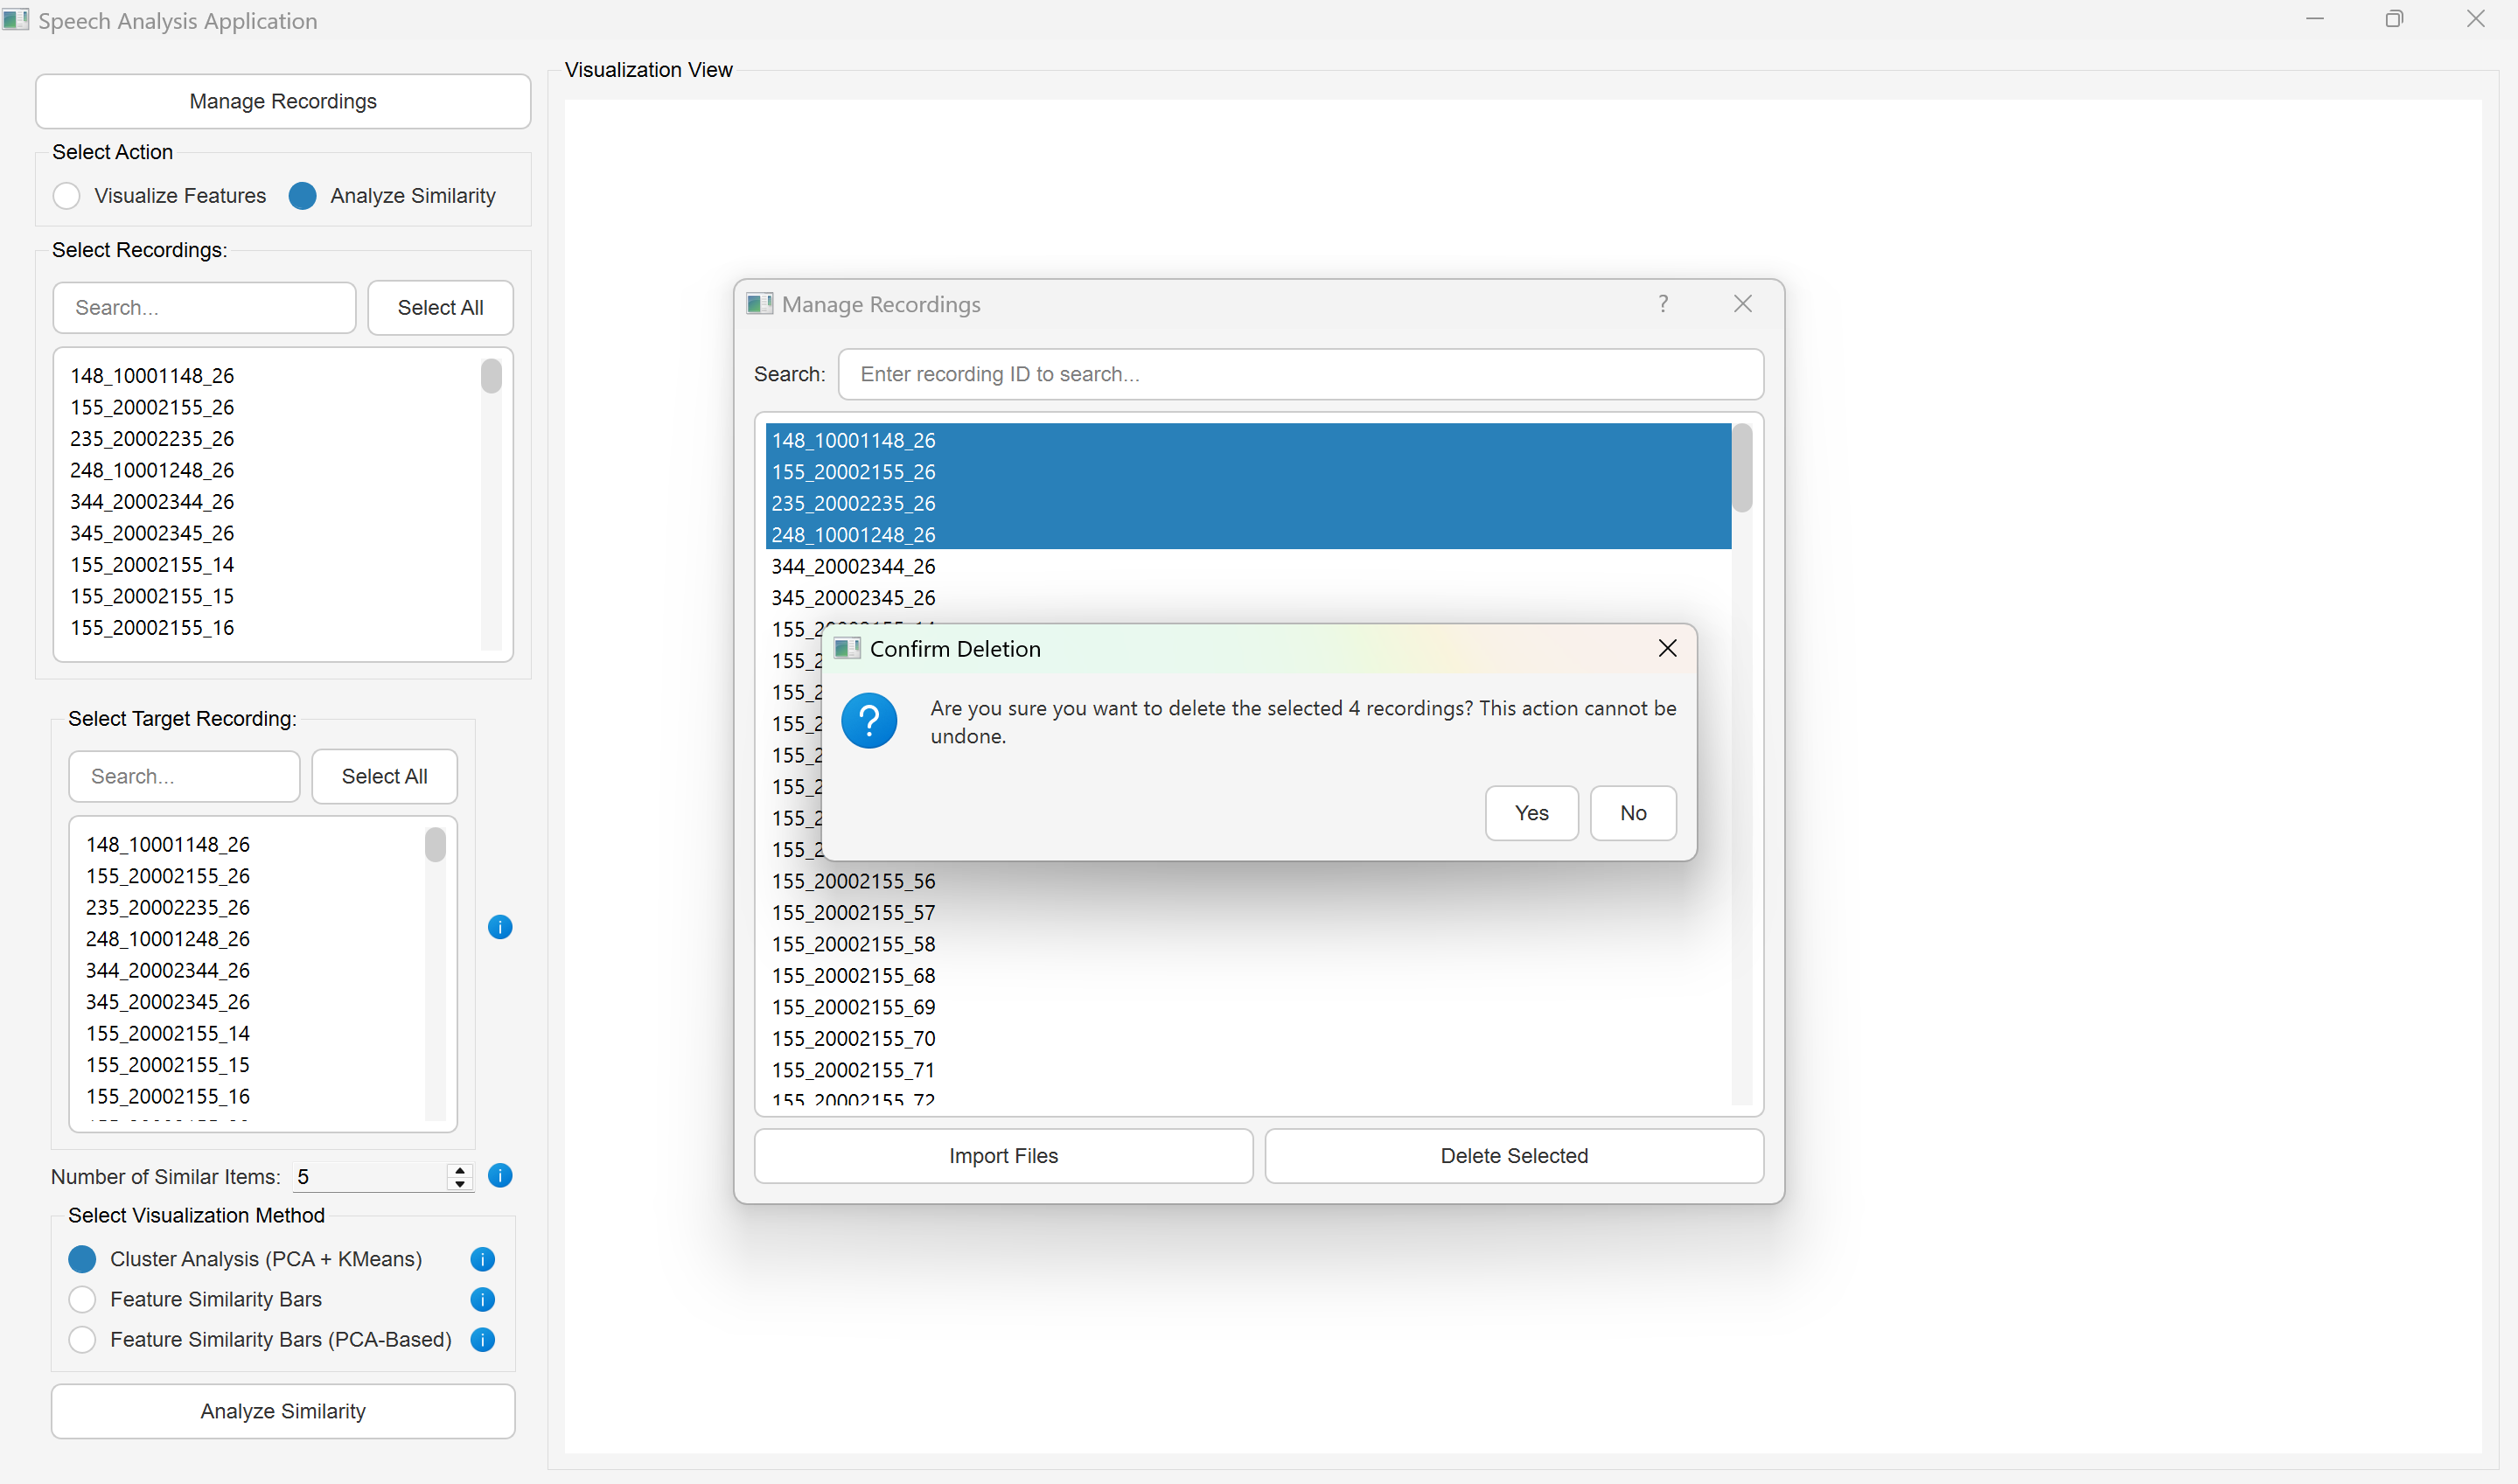
\includegraphics[width=\textwidth]{figures/rakenduse-teavitus-confirm.png}
    \caption{\textit{PCA koosinussarnasuse visualiseerimine tulpdiagrammil}}
    \label{fig:rakenduse-teavitus-confirm}
\end{figure}

\begin{figure}[ht]
    \centering
    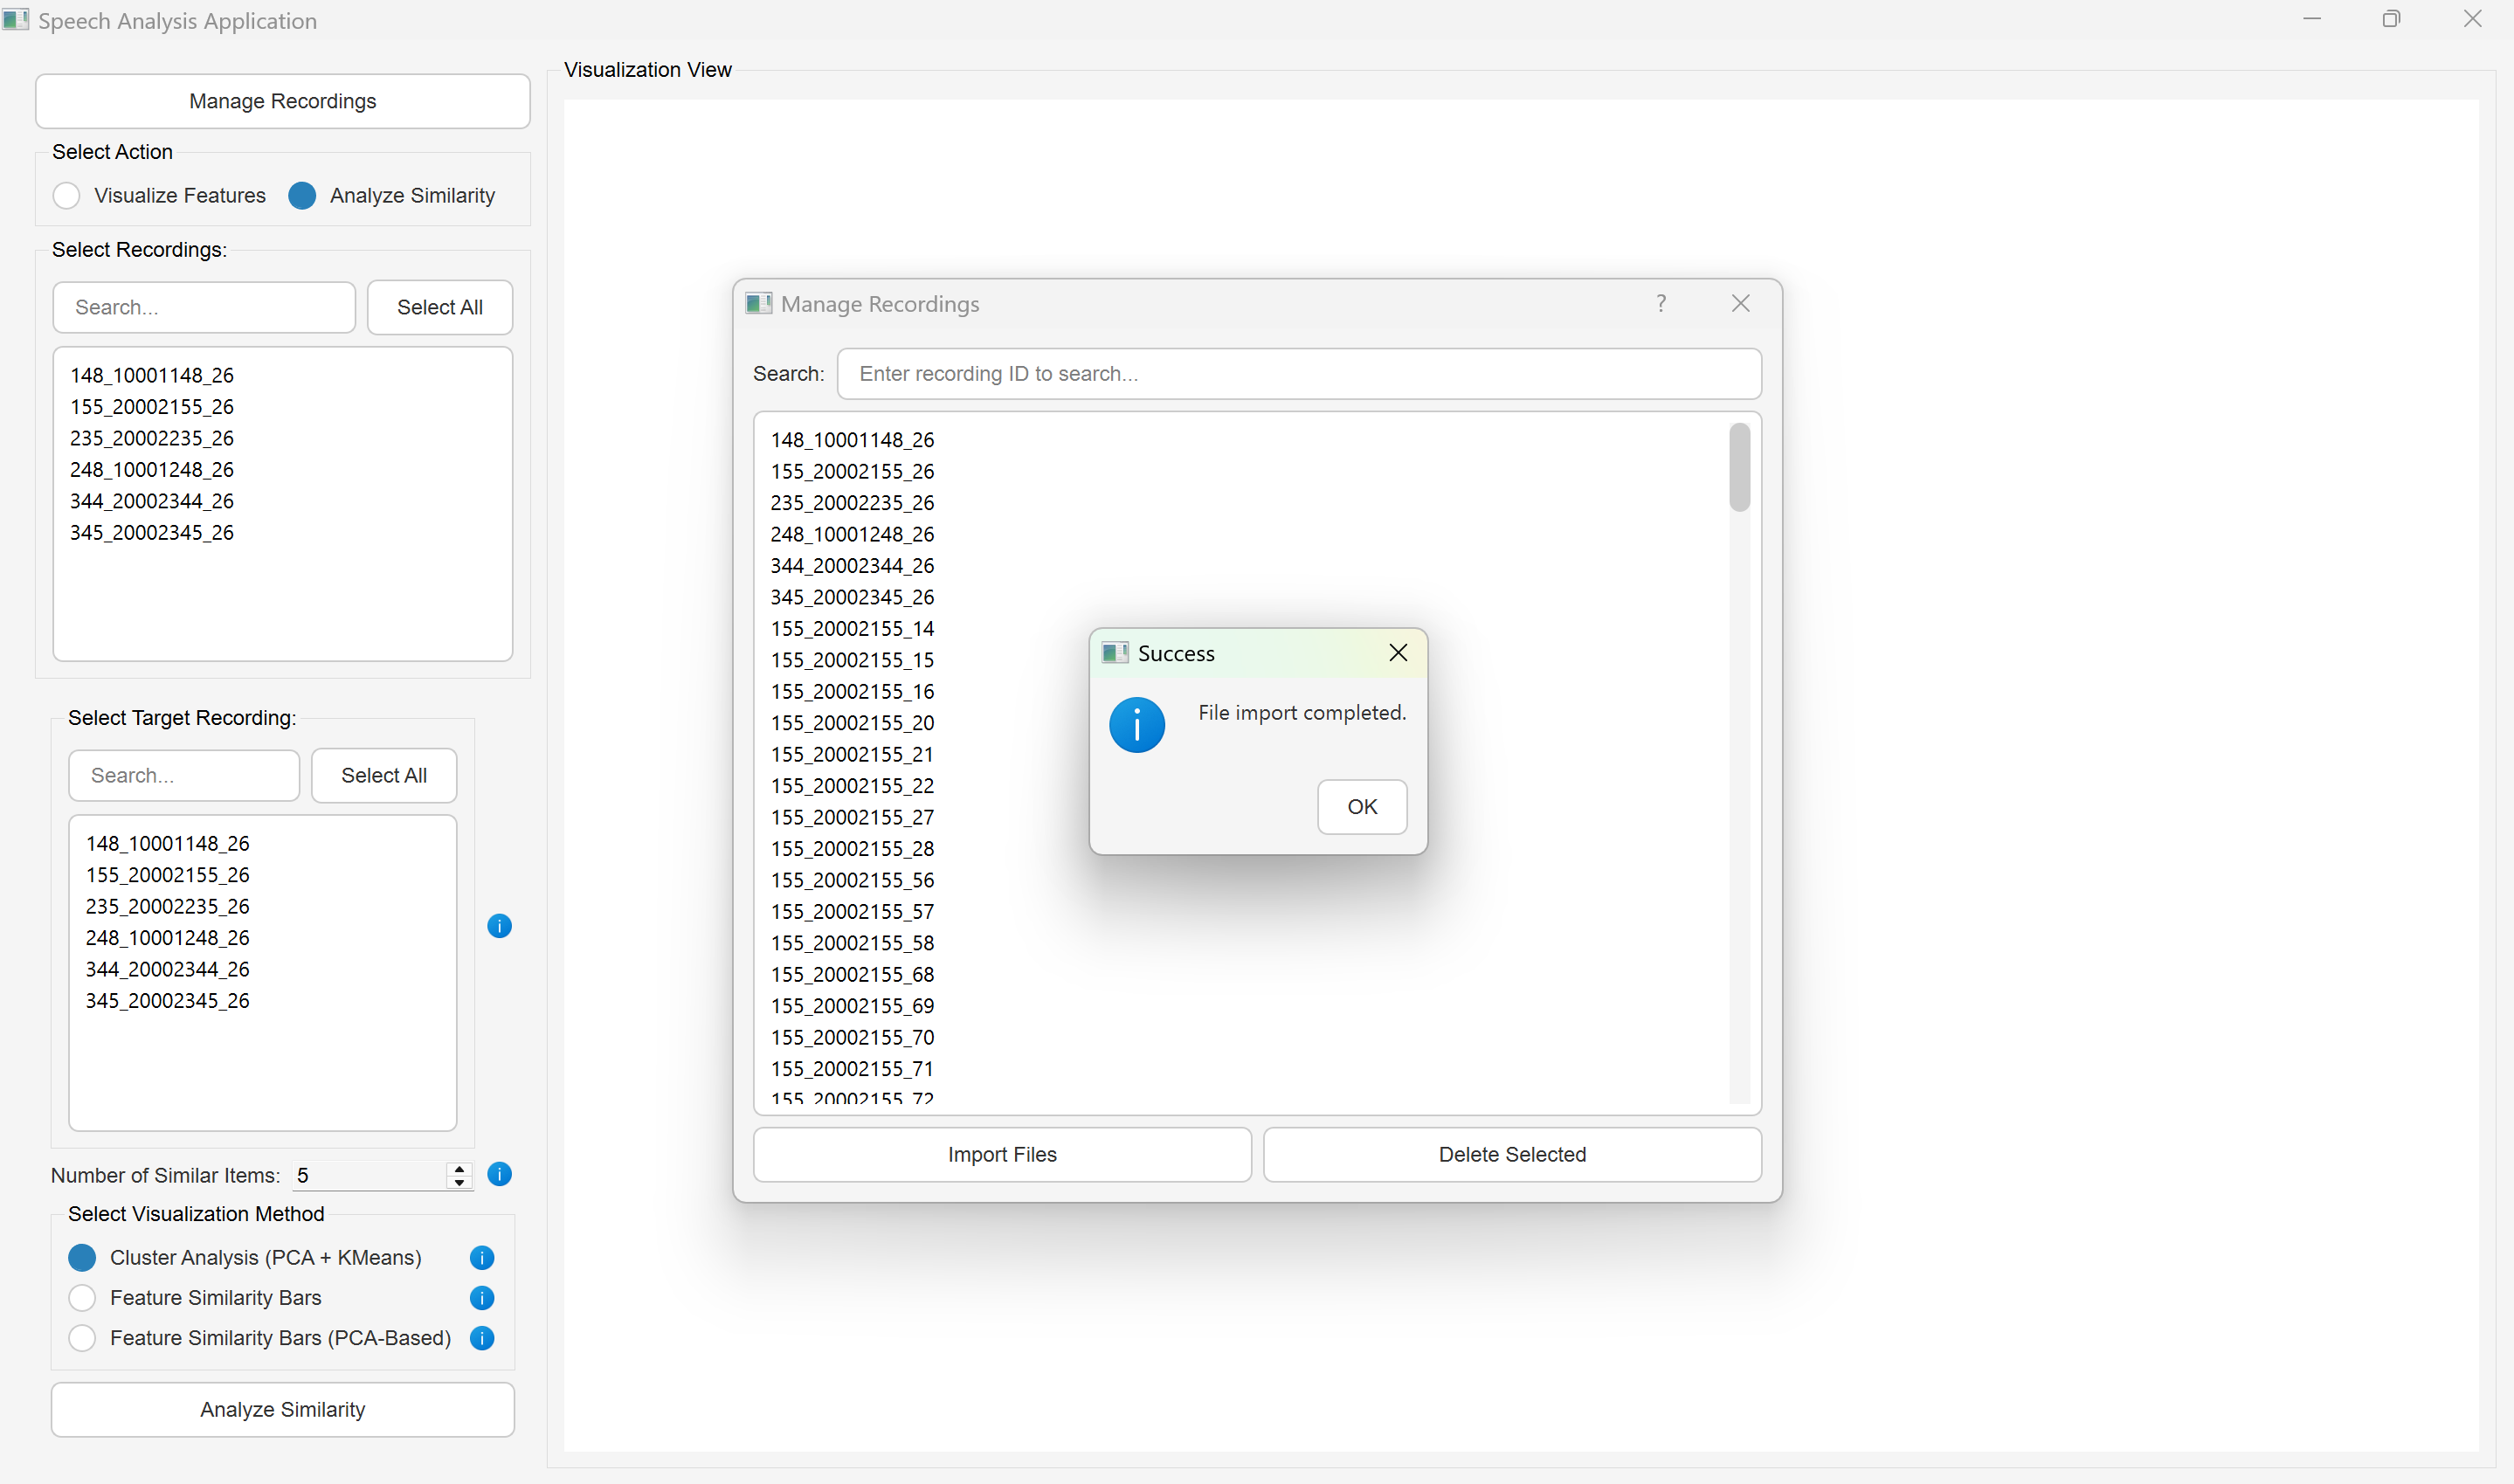
\includegraphics[width=\textwidth]{figures/rakenduse-teavitus-import-complete.png}
    \caption{\textit{Salvestuste andmete haldamise vaate impordi teavitus}}
    \label{fig:rakenduse-teavitus-confirm}
\end{figure}


\begin{figure}[ht]
    \centering
    \includegraphics[width=\textwidth]{figures/rakenduse-tunnus-sõna-timeline.png}
    \caption{\textit{Joondiagrammi näide ühe sõna ja tunnuse visualiseerimisel}}
    \label{fig:rakenduse-tunnus-sõna-timeline}
\end{figure}
\begin{figure}[ht]
    \centering
    \includegraphics[width=\textwidth]{figures/rakenduse-tunnus-sõna-histogram.png}
    \caption{\textit{Histogrammi näide ühe sõna ja tunnuse visualiseerimisel}}
    \label{fig:rakenduse-tunnus-sõna-histogram}
\end{figure}
\begin{figure}[ht]
    \centering
    \includegraphics[width=\textwidth]{figures/rakenduse-tunnus-2sõna-boxplot.png}
    \caption{\textit{Karpdiagrammi näide mitme sõna ja ühe tunnuse visualiseerimisel}}
    \label{fig:rakenduse-tunnus-sõna-boxplot}
\end{figure}
\begin{figure}[ht]
    \centering
    \includegraphics[width=\textwidth]{figures/rakenduse-tunnus-2sõna-radar.png}
    \caption{\textit{Radardiagrammi näide ühe mitme sõna ja tunnuse visualiseerimisel}}
    \label{fig:rakenduse-tunnus-2sõna-radar}
\end{figure}
\begin{figure}[ht]
    \centering
    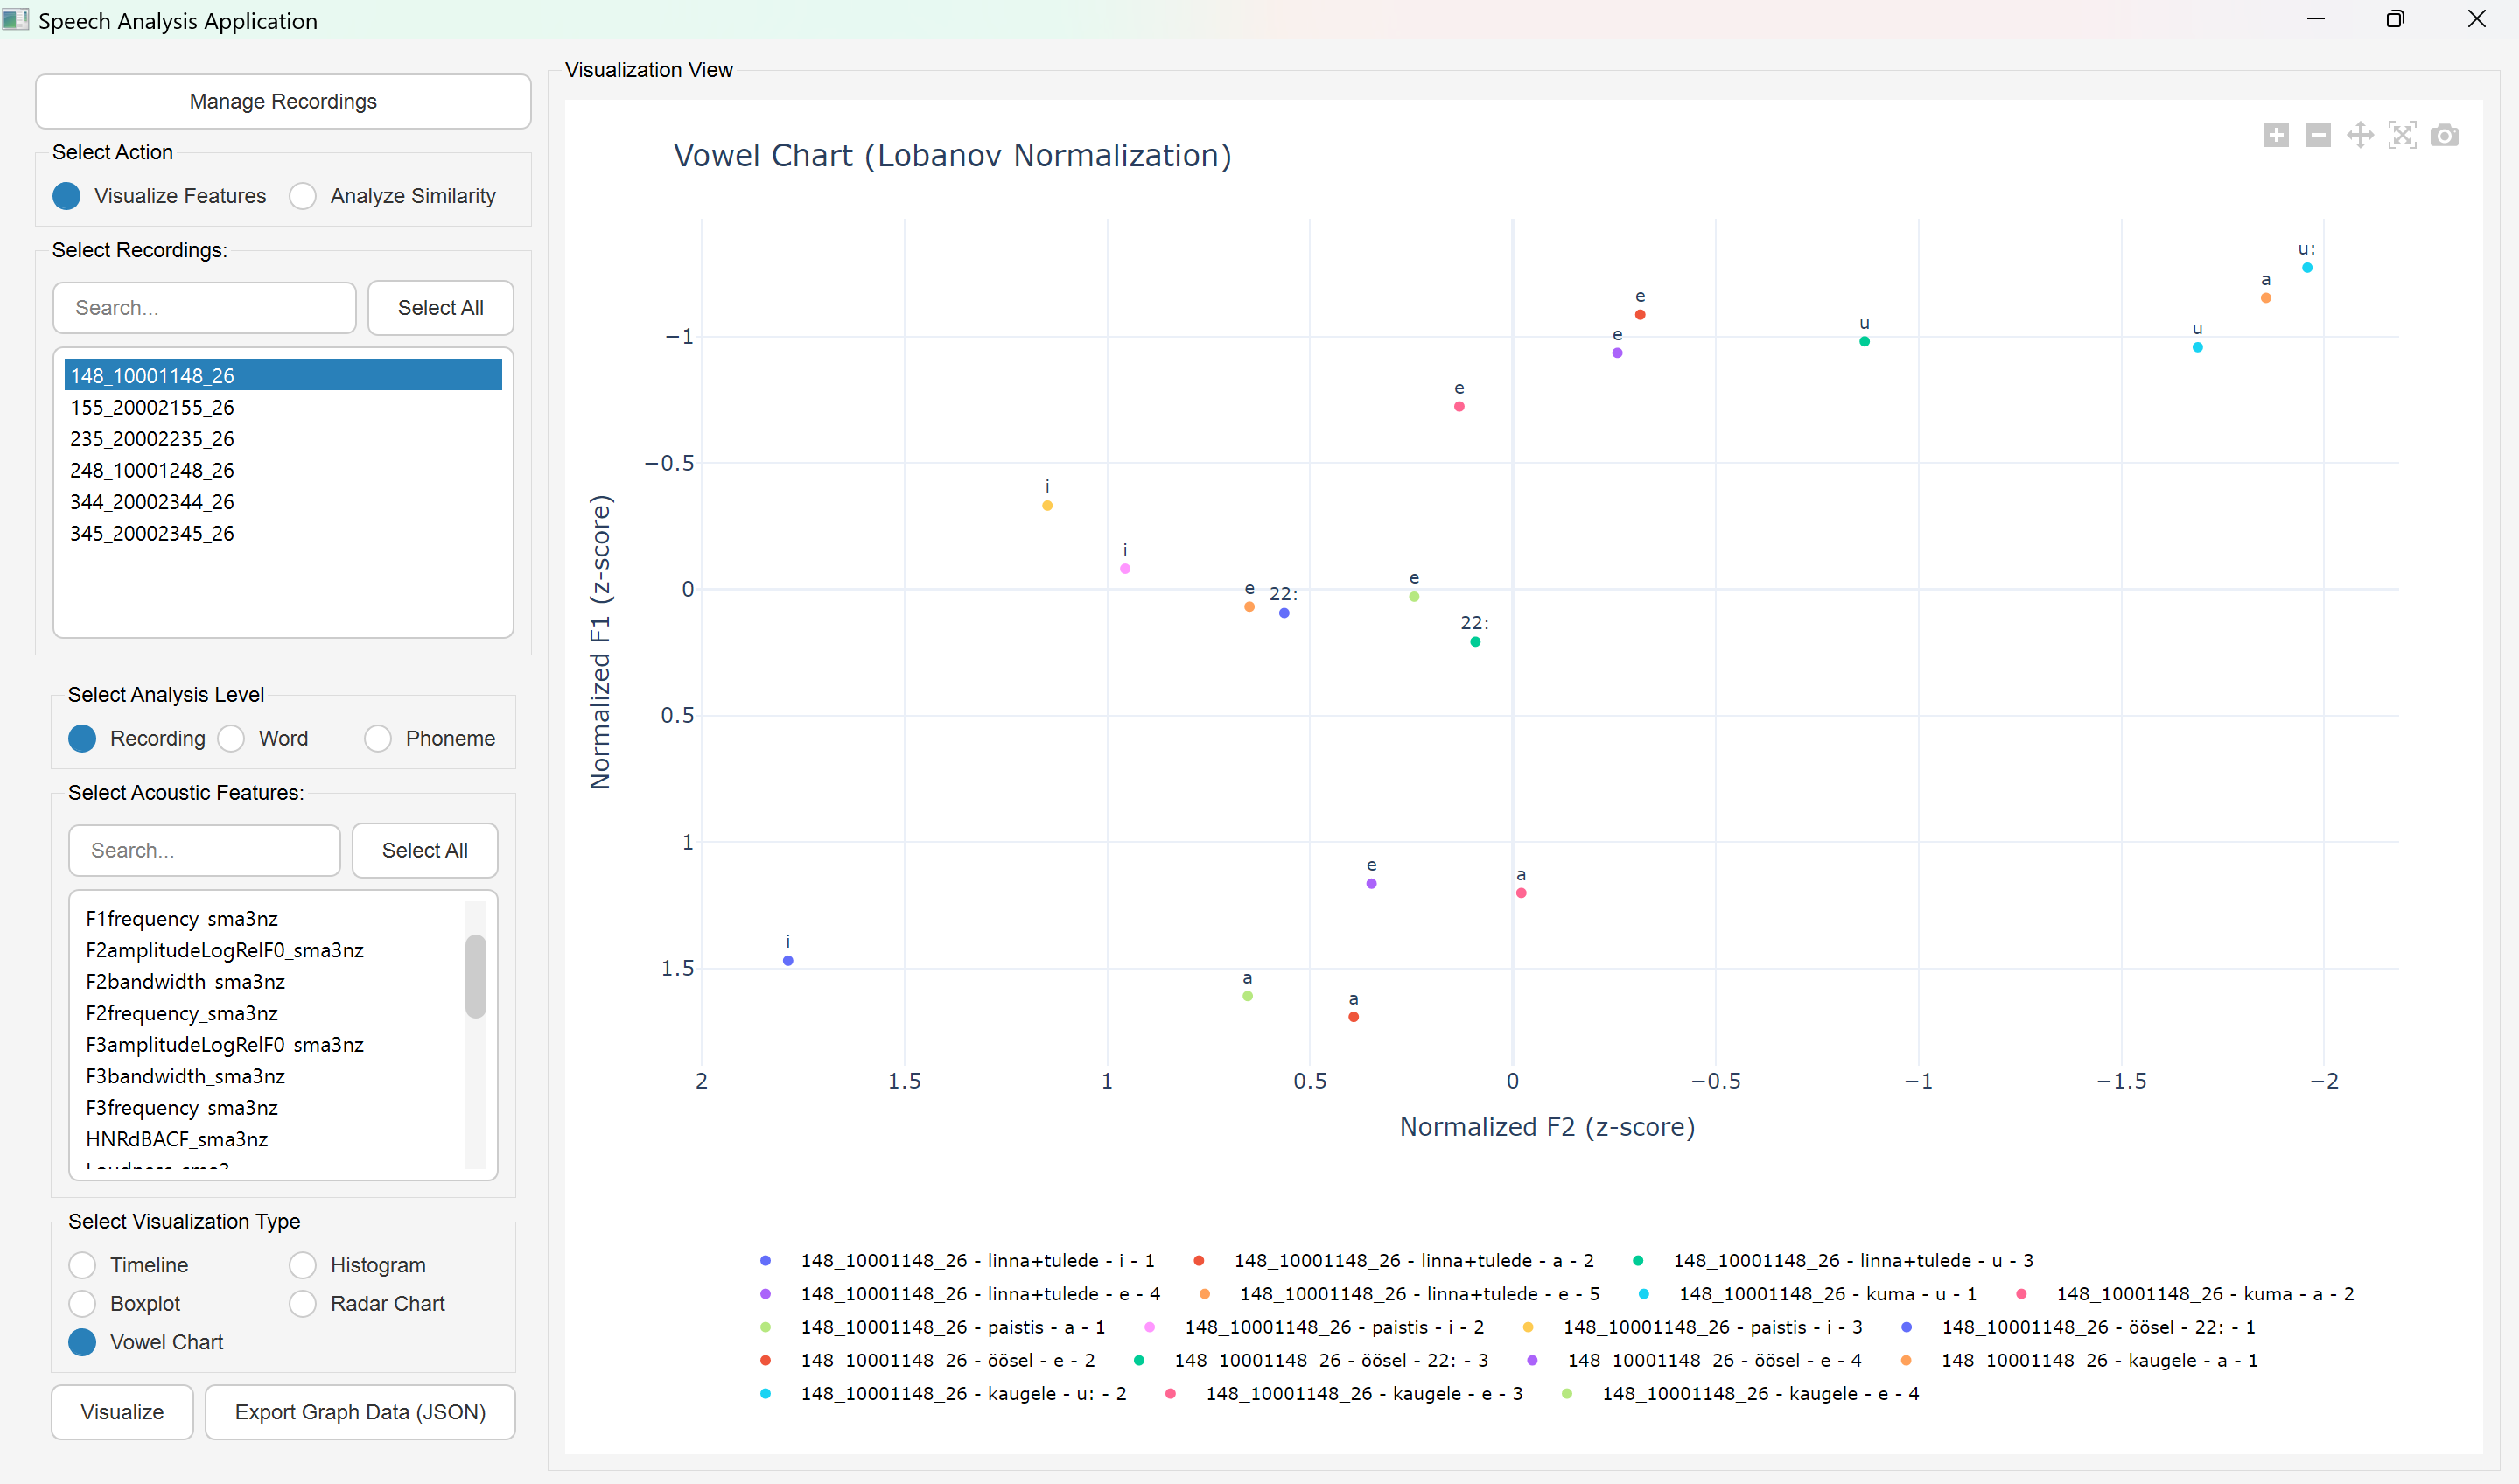
\includegraphics[width=\textwidth]{figures/rakenduse-tunnus-salvestus-vowel}
    \caption{\textit{Vokaalikaardi näide ühe salvestuse visualiseerimisel}}
    \label{fig:rakenduse-tunnus-salvestus-vowel}
\end{figure}

\begin{figure}[ht]
    \centering
    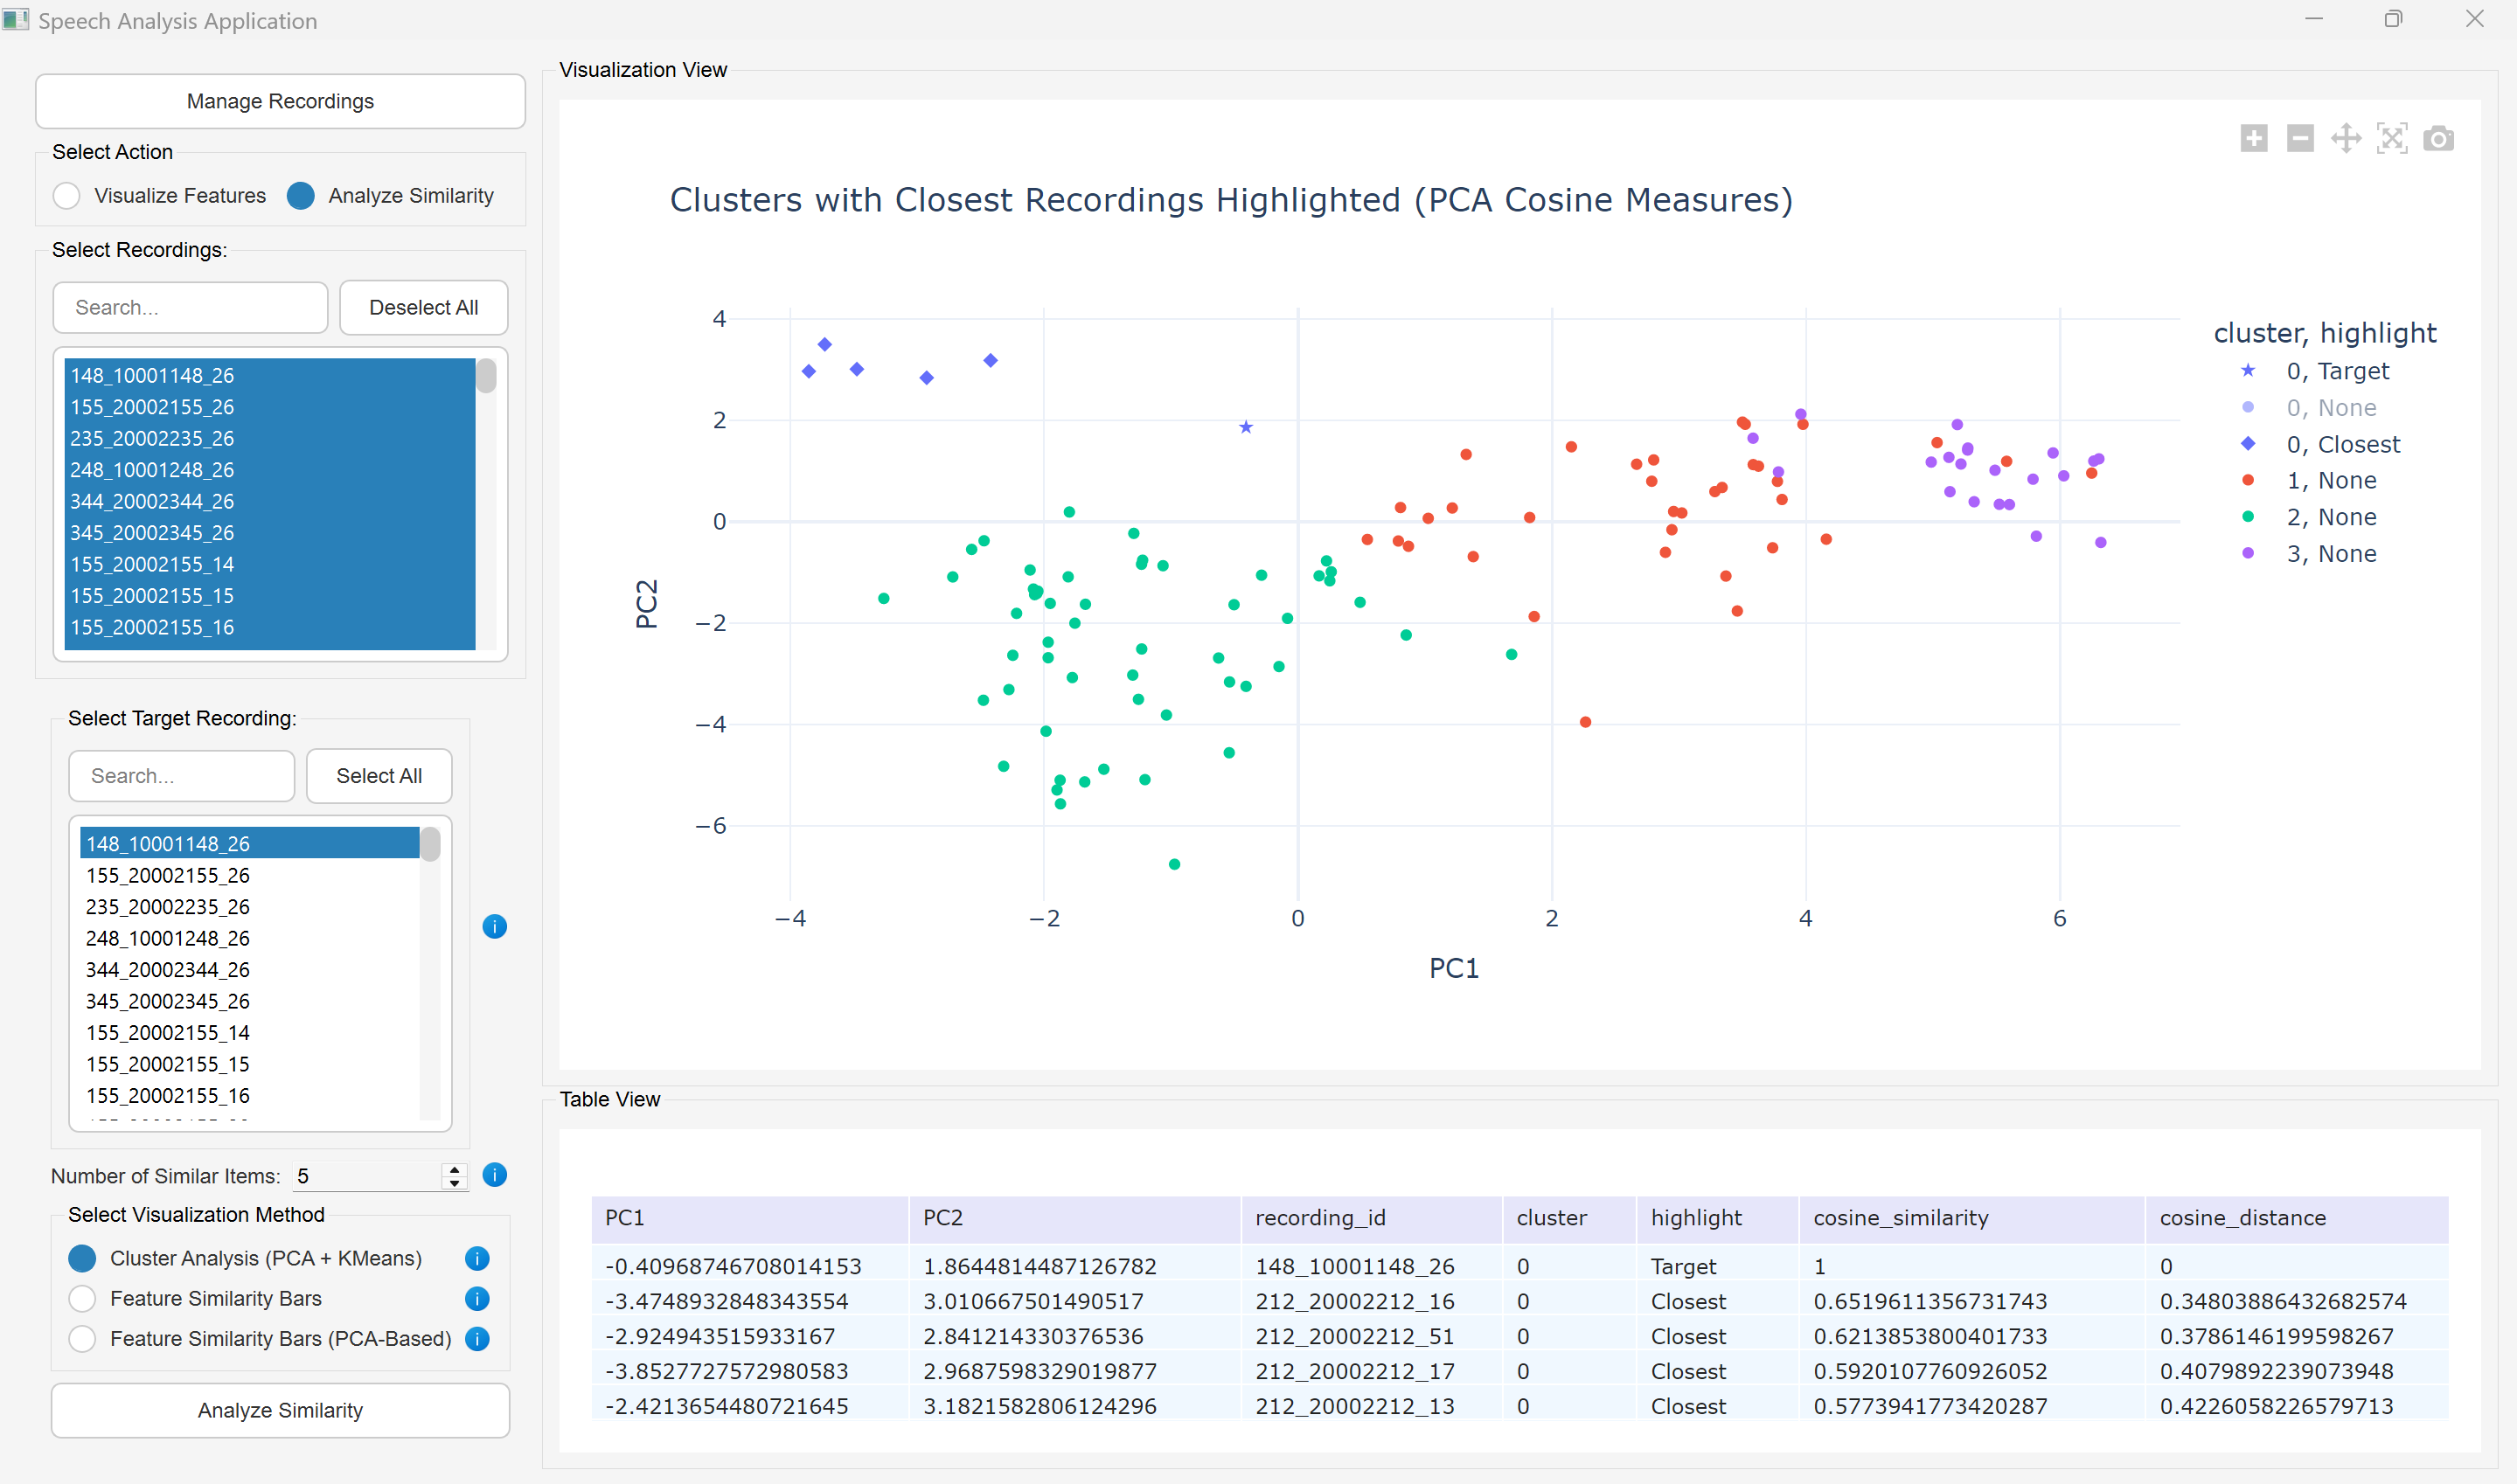
\includegraphics[width=\textwidth]{figures/rakenduse-sarnasus-cluster-closest.png}
    \caption{\textit{PCA koosinussarnasuse ja klastrite visualiseerimine hajuvusdiagrammil}}
    \label{fig:rakenduse-sarnasus-cluster-closest}
\end{figure}

\begin{figure}[ht]
    \centering
    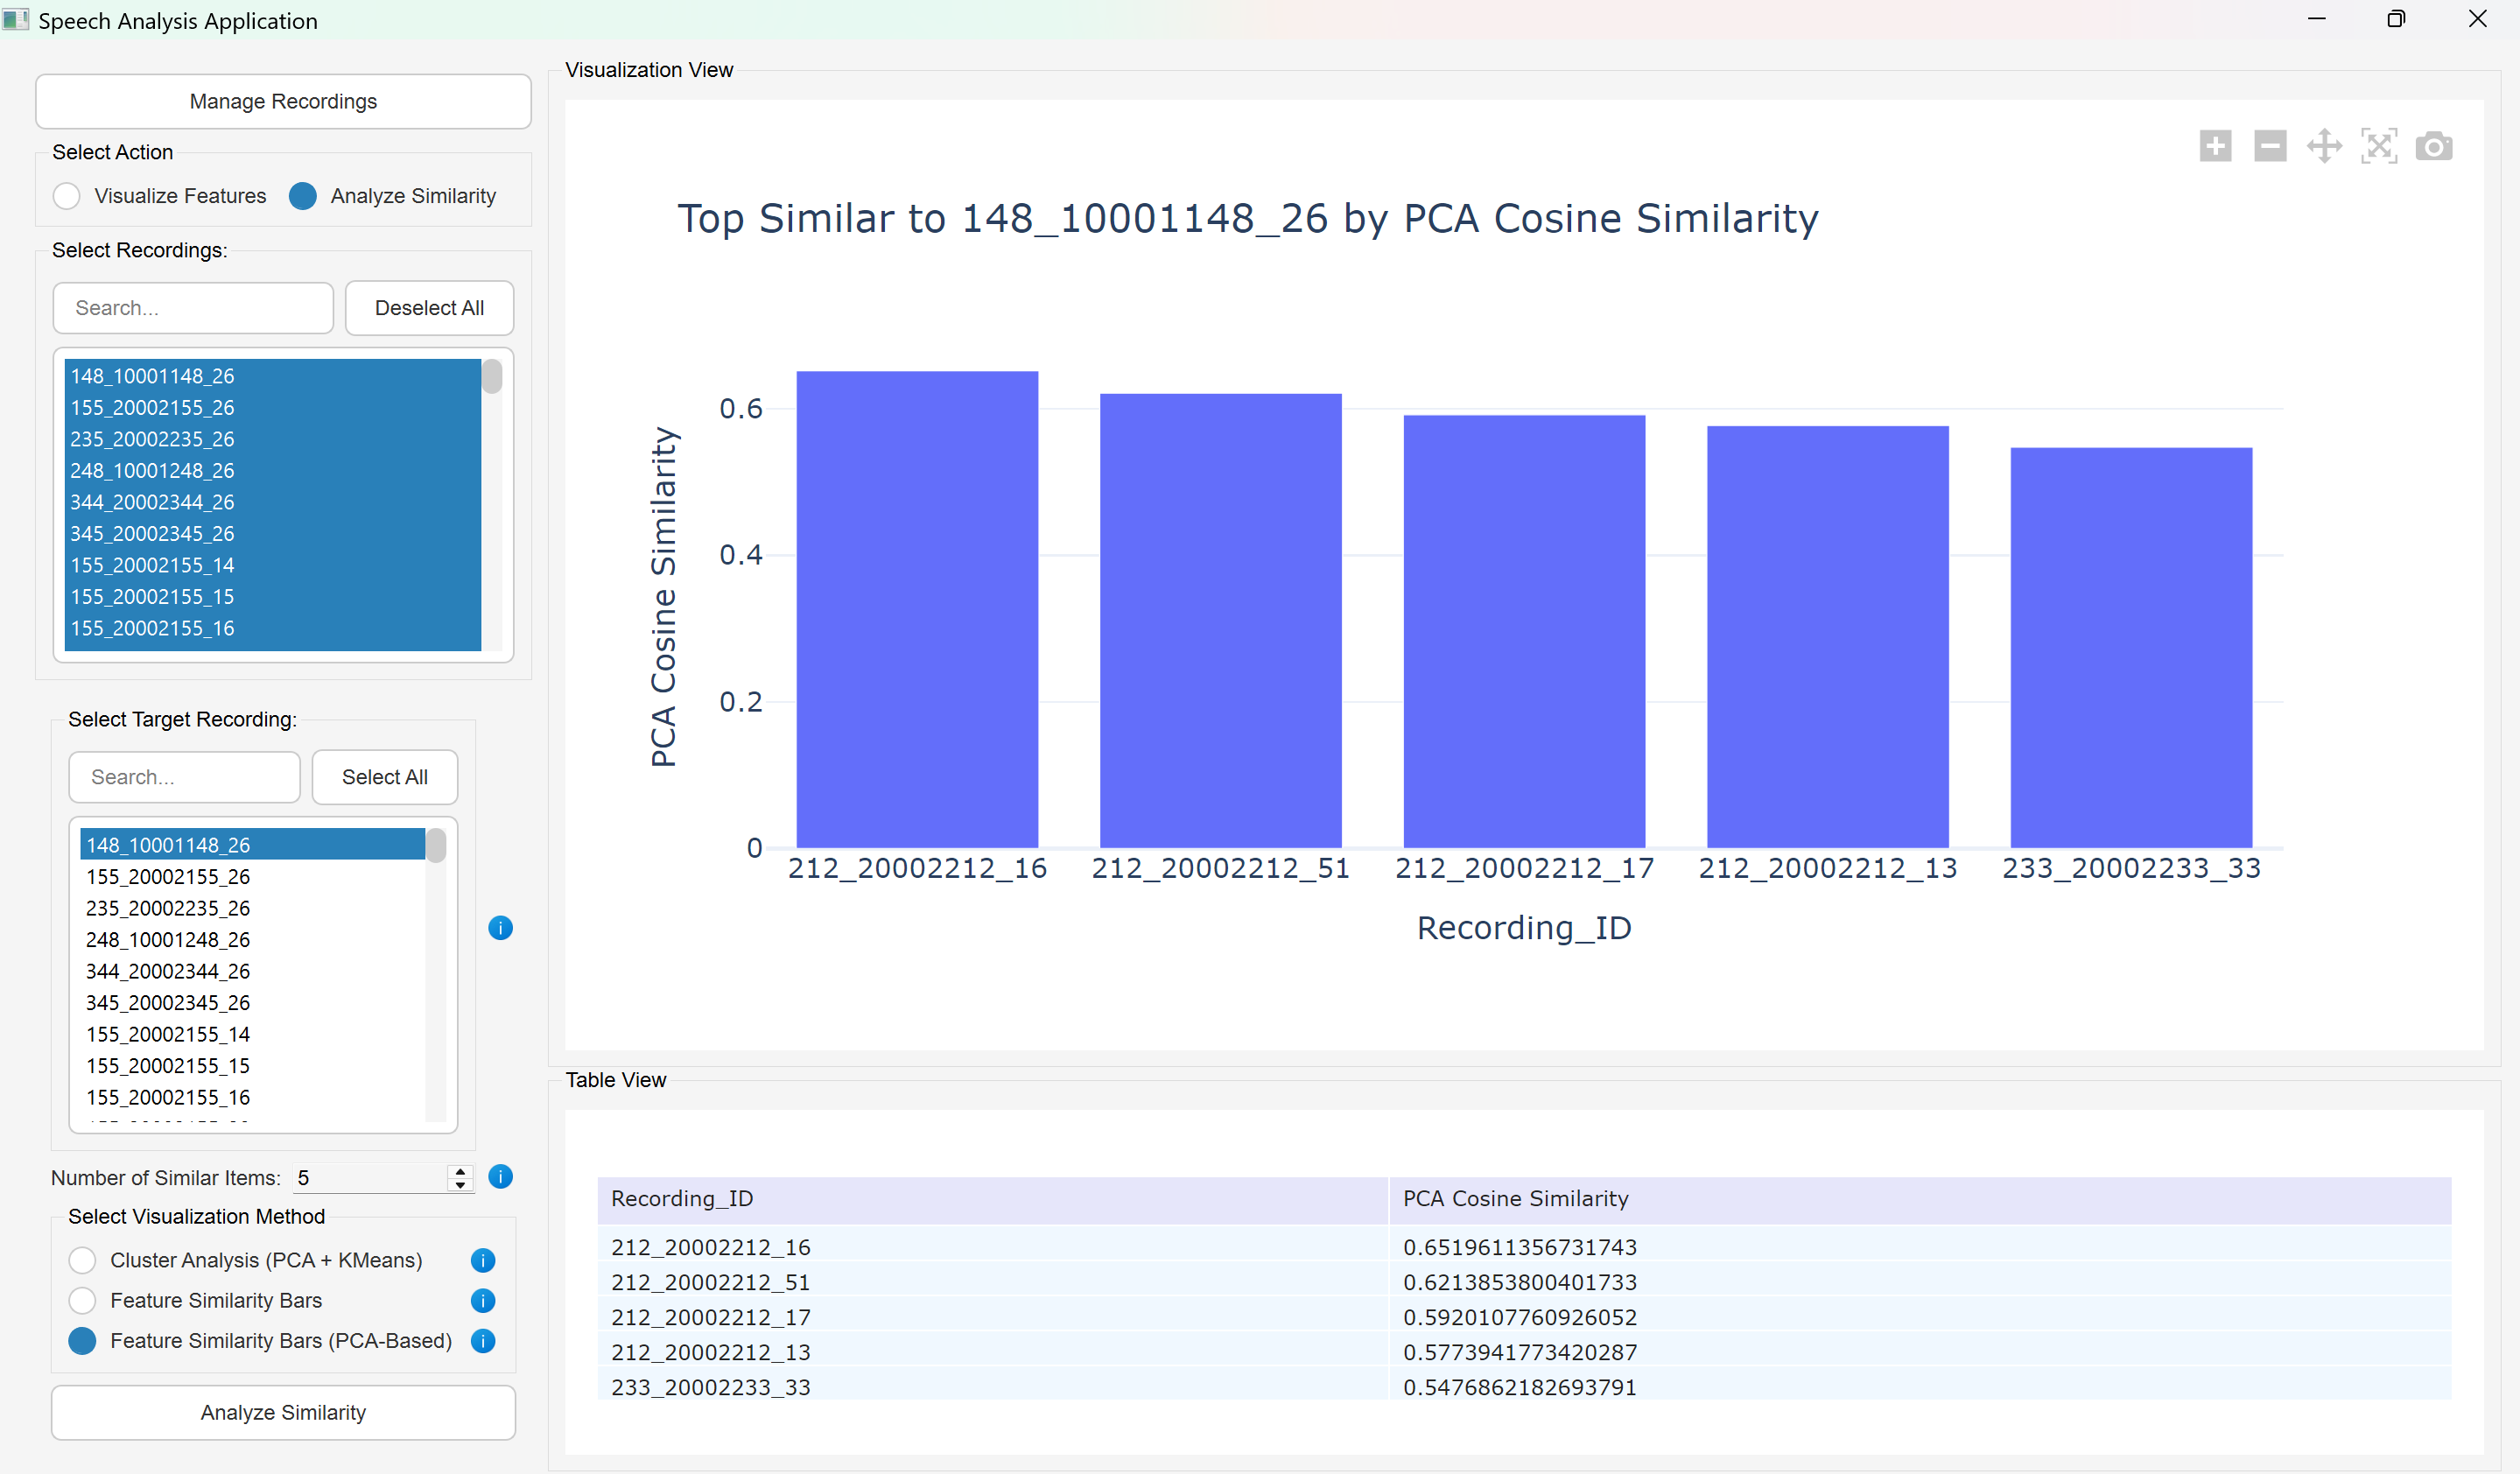
\includegraphics[width=\textwidth]{figures/rakenduse-sarnasus-pca-cosine.png}
    \caption{\textit{PCA koosinussarnasuse visualiseerimine tulpdiagrammil}}
    \label{fig:rakenduse-sarnasus-pca-cosine}
\end{figure}

\begin{figure}[ht]
    \centering
    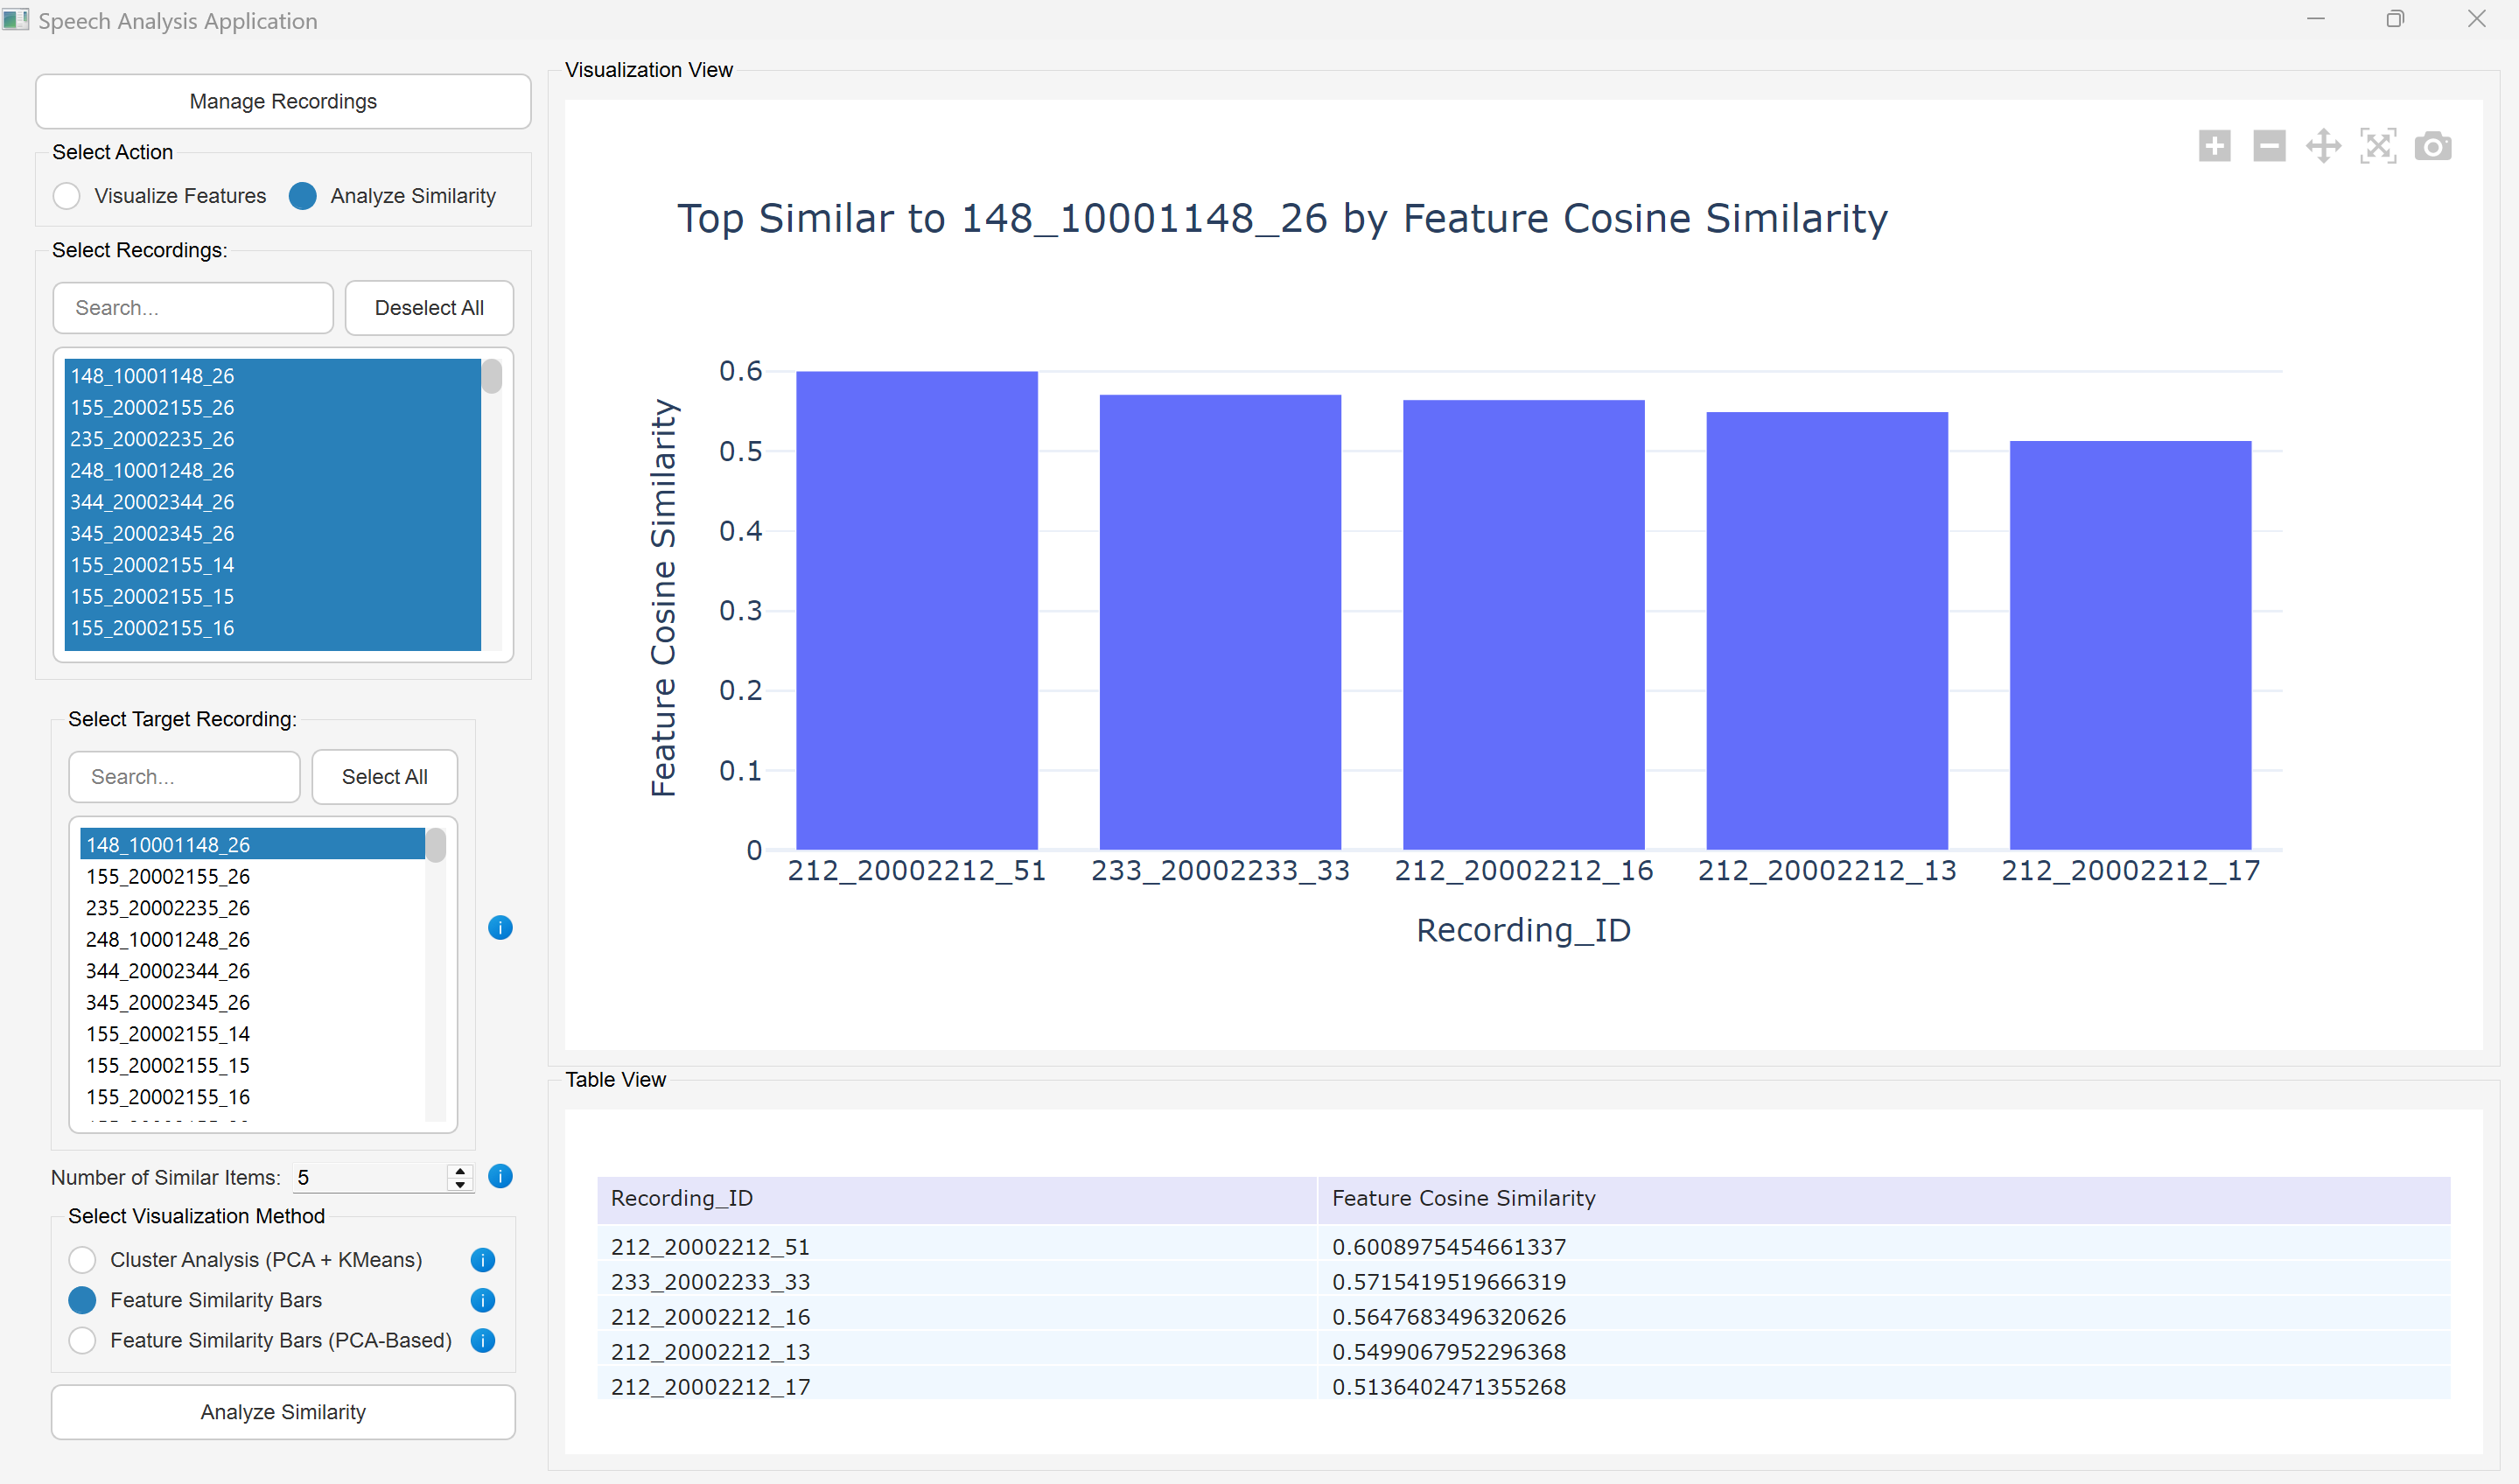
\includegraphics[width=\textwidth]{figures/rakenduse-sarnasus-cosine.png}
    \caption{\textit{Koosinussarnasuse visualiseerimine tulpdiagrammil}}
    \label{fig:rakenduse-sarnasus-cosine}
\end{figure}


\clearpage
\phantomsection
\addcontentsline{toc}{chapter}{Lisa 4 -- Kõne tunnuste analüüsimise rakenduse tagasiside küsimustik}\label{chapter:Lisa 2}
\chapter*{Lisa 4 - Tagasiside küsimused}
Tere! Olen Hanna Raudsepp, Tallinna Tehnikaülikooli informaatika eriala bakalaureuseõppe tudeng. Minu lõputööks on "Hääle akustiliste tunnuste visualiseerimise rakendus" ning selle eesmärk on luua tööriist, mis võimaldab kõnesalvestuste akustiliste tunnuste analüüsi ja visuaaliseerimist.

Küsimustik on koostatud, et koguda tagasisidet rakenduse funktsionaalsuse ja kasutajamugavuse kohta.

Küsimused:

\begin{enumerate}
    \item Kas tegelete foneetika või kõne uurimisega?
    \item Kas rakenduse loodud graafikud olid arusaadavad ja kasulikud? (Rakenduse graafikud: ajagraafik, histogramm, karpdiagram, radar, vokaalikaart, sarnaste salvestuste klaster, sarnaste salvestuste tulpdiagrammid) 
    \item Kas märkasite rakenduse kasutamisel tehnilisi probleeme või tõrkeid? Kui jah, siis milliseid?
    \item Hinnake skaalal 1–5, kui kasutajasõbralik ja mugav oli rakenduse kasutamine teie arvates? 1 = „väga ebamugav“, 5 = „väga mugav“. Selgitage oma hinnangut.
    \item Millised rakenduse funktsioonid tundusid teie jaoks kõige kasulikumad?
    \item Milliseid täiustusi või lisafunktsioone soovitaksite rakendusele lisada?
    \item Muud kommentaarid
\end{enumerate}


